\section*{Porównanie wyników eksperymentów symulacyjnych oraz z wykorzystaniem rzeczywistych robotów}
\begin{frame}
\frametitle{\secname}
\framesubtitle{Otwarta przestrzeń ustawienie prostopadłe}
\begin{figure}[ht] % h:here; t:top; b:bottom; p:page; default:ht
	\captionsetup[subfigure]{labelformat=empty}
	\centering
	\subfloat[][Symulacja 1-2]
{
	\includegraphics[page = 2, width=0.49\textwidth]{img/Simulation_Open_space.pdf}
}
	\subfloat[][Roboty 1-2]
{
	\includegraphics[page = 2, width=0.49\textwidth]{img/Robots_Open_space.pdf}
}
\end{figure}
\end{frame}


\section*{Porównanie wyników eksperymentów symulacyjnych oraz z wykorzystaniem rzeczywistych robotów}
\begin{frame}
\frametitle{\secname}
\framesubtitle{Przejście przez drzwi}
\begin{figure}[ht] % h:here; t:top; b:bottom; p:page; default:ht
	\captionsetup[subfigure]{labelformat=empty}
	\centering
		\subfloat[][Symulacja 1-H2]
{
	\includegraphics[page = 2, width=0.49\textwidth]{img/Simulation_Passage_through_the_door.pdf}
}
	\subfloat[][Roboty 1-H2]
{
	\includegraphics[page = 2, width=0.49\textwidth]{img/Robots_Passage_through_the_door.pdf}
}
\end{figure}
\end{frame}
